%
%

%%-----------------------------------------------------
%%-----------------------------------------------------
\section{La maravillosa Wayback Machine}

%%-----------------------------------------------------
\begin{frame}
\frametitle{¿Cómo era la web de la URJC?}


\includegraphics[height=6cm]{figs/web-urjc-2014}

{\Large
\begin{flushright}
2014
\end{flushright}
}
\end{frame}

%%-----------------------------------------------------
\begin{frame}
\frametitle{¿Cómo era la web de la URJC?}

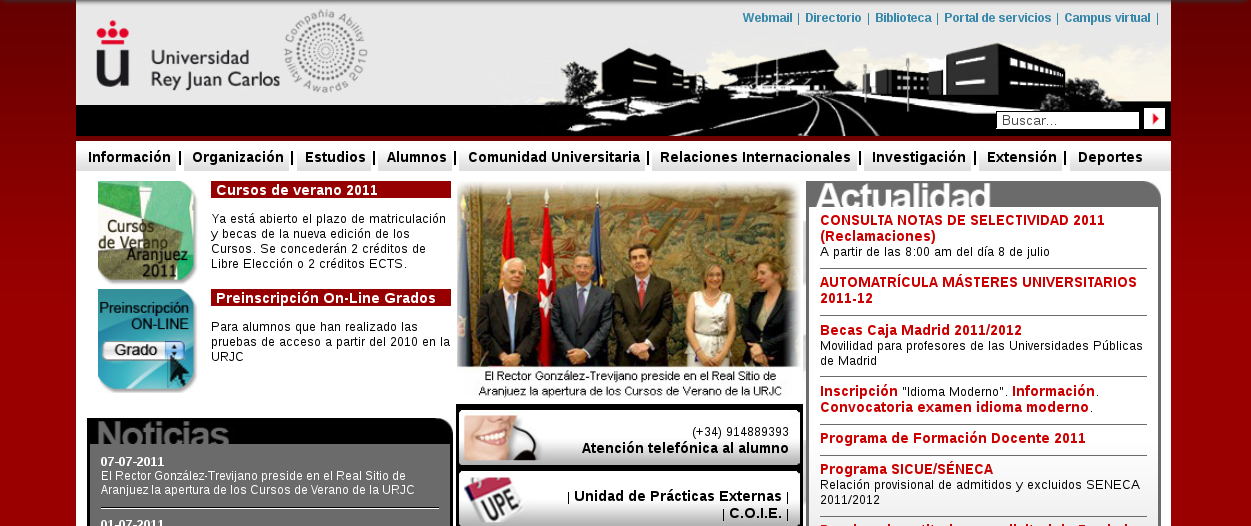
\includegraphics[height=6cm]{figs/web-urjc-2011}

{\Large
\begin{flushright}
2011
\end{flushright}
}
\end{frame}

%%-----------------------------------------------------
\begin{frame}
\frametitle{¿Cómo era la web de la URJC?}

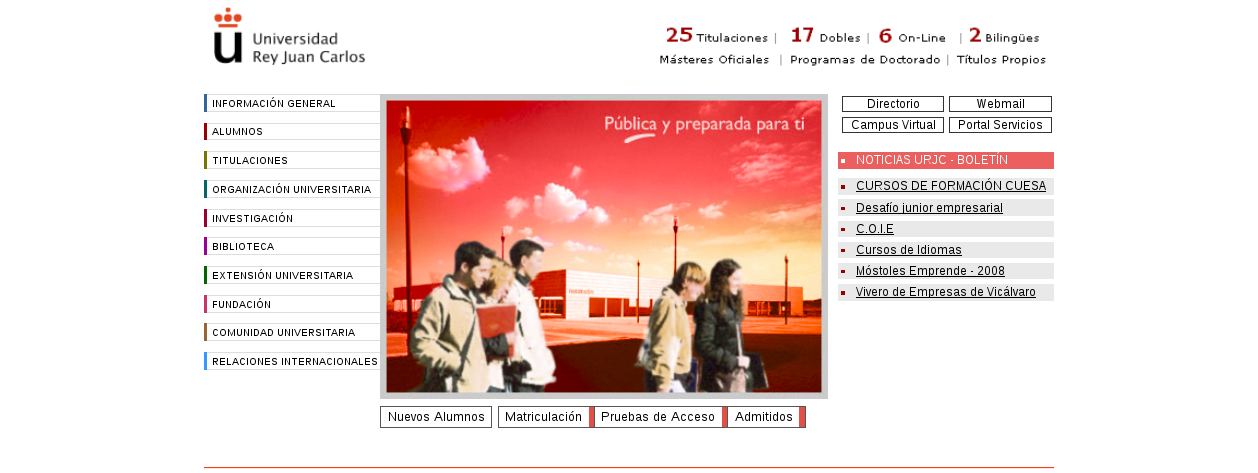
\includegraphics[height=6cm]{figs/web-urjc-2008}

{\Large
\begin{flushright}
2008
\end{flushright}
}
\end{frame}

%%-----------------------------------------------------
\begin{frame}
\frametitle{¿Cómo era la web de la URJC?}

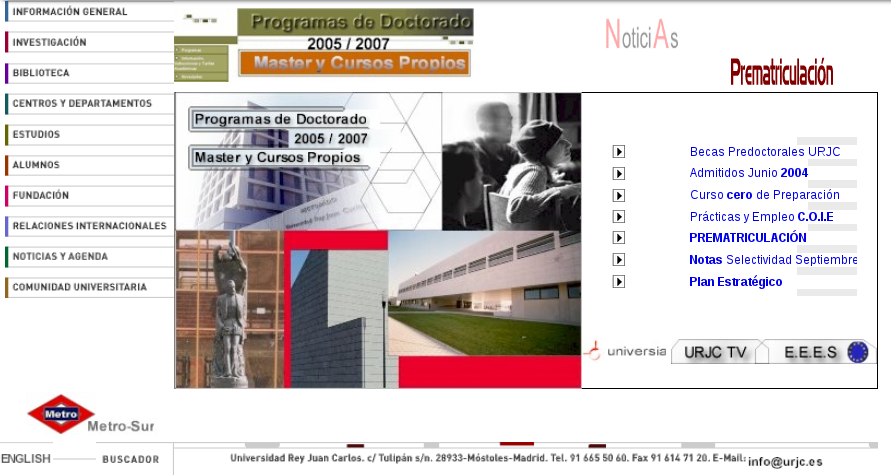
\includegraphics[height=6cm]{figs/web-urjc-2004}

{\Large
\begin{flushright}
2004
\end{flushright}
}
\end{frame}

%%-----------------------------------------------------
\begin{frame}
\frametitle{Bienvenidos a la maravillosa Wayback Machine}

{\Large
\begin{itemize}
\item Copias sitios web en distintos momentos del pasado
\item Parte del Internet Archive
\item Proporiciona una interfaz web...
\item ...y una API
\end{itemize}

\begin{flushright}
\url{https://archive.org/web/} \\
\url{https://archive.org/help/wayback_api.php} \\
\end{flushright}

\begin{itemize}
\item Otra opción: Screenshots.com \\
  \url{http://www.screenshots.com} \\
\item Memmento: acceso a el pasado \\
  \url{http://www.mementoweb.org/} \\
\end{itemize}
}


\end{frame}


